%% IEEE INFOCOM 2027 -- Demo track (2-page abstract, IEEE format, single-blind)
%% Draft v3 -- Cross-Domain Conflict Guard
%% Restructured to the INFOCOM'26 XR-QoD demo template (Intro / Architecture /
%% Demo Description & Results / Conclusion) + SymbXRL booth-walkthrough & setup blocks.
%% Compile: pdflatex conflict-guard-abstract.tex (needs IEEEtran.cls + tikz; run twice for refs)
\documentclass[conference]{IEEEtran}
\usepackage{cite}
\usepackage{graphicx}
\usepackage{amsmath}
\usepackage{url}
\usepackage{tikz}
\usetikzlibrary{positioning,arrows.meta,fit,backgrounds,calc}

\begin{document}

\title{Demo: You Cannot Guarantee QoS on a Sleeping Cell---%
Cross-Domain Conflict Guarding in an NWDAF-Extended 5G Control Plane}

%% Single-blind: fill in real author names before submission.
\author{\IEEEauthorblockN{[Author Names]}
\IEEEauthorblockA{Electronics and Telecommunications Research Institute (ETRI)\\
Daejeon, Republic of Korea\\
Email: \{...\}@etri.re.kr}}

\maketitle

\begin{abstract}
This demo presents a live closed-loop \emph{cross-domain conflict guard} for an
NWDAF-extended 5G analytics-and-control function (NCOF). From a single shared
signal---non-3GPP (WLAN) downlink throughput---NCOF drives two heterogeneous
control loops at once: RAN energy, by placing a small-cell gNB into
\texttt{DEEP\_SLEEP} through a RAN control function (RICF), and core QoS, by
updating guaranteed/maximum downlink bitrate at the PCF. Because both decisions
originate in one function and act on the same cell, they can conflict in a way
no RAN-only mitigator nor any single core NF can observe: the function may
guarantee a bitrate on a cell it is simultaneously deactivating. The Conflict
Guard (i) reads each incoming subscription with an LLM to flag semantically
antagonistic intents at subscription time, and (ii) re-checks a compatibility
predicate over pending actuations before dispatch, deferring commands under a
declared precedence policy. Running on a five-NF prototype with a real-time
dashboard, the demo lets attendees induce the conflict and watch the guard
close a concrete QoS-violation window live.
\end{abstract}

\begin{IEEEkeywords}
5G core, NWDAF, service exposure, closed-loop control, energy saving, QoS,
conflict mitigation, large language models, Demo.
\end{IEEEkeywords}

\begin{figure*}[!t]
\centering
\resizebox{\textwidth}{!}{%
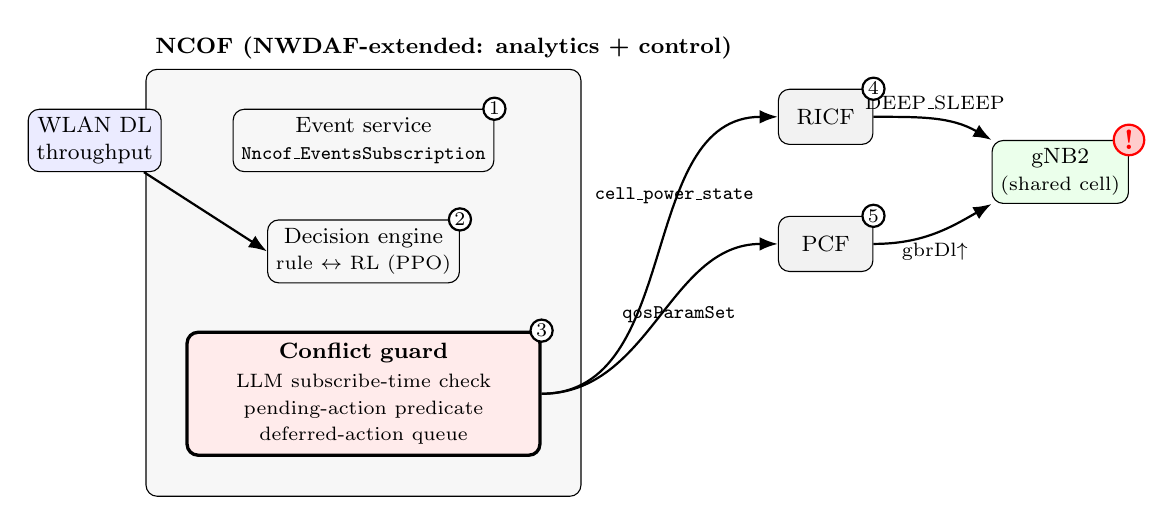
\begin{tikzpicture}[
  font=\footnotesize,
  box/.style={draw,rounded corners,align=center,minimum height=7mm,inner sep=3pt},
  nf/.style={draw,rounded corners,fill=black!5,align=center,minimum height=7mm,minimum width=12mm},
  guard/.style={draw,very thick,rounded corners,fill=red!8,align=center,inner sep=4pt,text width=42mm},
  sig/.style={-{Latex},thick},
  badge/.style={circle,draw,thick,fill=white,inner sep=0.7pt,font=\scriptsize},
]
\node[box,fill=blue!8] (wlan) {WLAN DL\\throughput};
\node[box,right=9mm of wlan] (es) {Event service\\{\scriptsize\ttfamily Nncof\_EventsSubscription}};
\node[box,below=6mm of es] (de) {Decision engine\\{\scriptsize rule $\leftrightarrow$ RL (PPO)}};
\node[guard,below=6mm of de] (cg) {\textbf{Conflict guard}\\[1pt]%
{\scriptsize LLM subscribe-time check}\\%
{\scriptsize pending-action predicate}\\%
{\scriptsize deferred-action queue}};
\begin{scope}[on background layer]
\node[draw,rounded corners,fill=black!3,inner sep=5mm,fit=(es)(de)(cg)] (ncof) {};
\end{scope}
\node[anchor=south west,font=\footnotesize\bfseries] at (ncof.north west)
  {NCOF (NWDAF-extended: analytics + control)};
\draw[sig] (wlan) -- (de.west);

\node[nf,right=36mm of es,yshift=3mm] (ricf) {RICF};
\node[nf,below=9mm of ricf] (pcf) {PCF};
\node[box,fill=green!8,right=15mm of ricf,yshift=-7mm] (gnb) {gNB2\\{\scriptsize (shared cell)}};

\draw[sig] (cg.east) to[out=0,in=180]
  node[pos=0.6,above,font=\scriptsize]{\ttfamily cell\_power\_state} (ricf.west);
\draw[sig] (cg.east) to[out=0,in=180]
  node[pos=0.6,below,font=\scriptsize]{\ttfamily qosParamSet} (pcf.west);
\draw[sig] (ricf.east) to[out=0,in=150]
  node[pos=0.5,above,font=\scriptsize]{DEEP\_SLEEP} (gnb.north west);
\draw[sig] (pcf.east) to[out=0,in=210]
  node[pos=0.5,below,font=\scriptsize]{gbrDl$\uparrow$} (gnb.south west);
\node[circle,draw=red,thick,fill=red!20,text=red,font=\bfseries,inner sep=1.2pt]
  at (gnb.north east) {!};

%% numbered callouts (SymbXRL-style)
\node[badge] at (es.north east) {1};
\node[badge] at (de.north east) {2};
\node[badge] at (cg.north east) {3};
\node[badge] at (ricf.north east) {4};
\node[badge] at (pcf.north east) {5};
\end{tikzpicture}%
}
\caption{NCOF (an NWDAF-extended analytics+control function) drives two
cross-domain closed loops from one signal. (1)~event-subscription service,
(2)~rule/RL decision engine, (3)~the Conflict Guard, (4)~RAN power loop via
RICF, (5)~core QoS loop via PCF. The guard sits between the decision engine and
the notification senders; PCF and RICF are NCOF event-subscription consumers.}
\label{fig:arch}
\end{figure*}

\section{Introduction}
Analytics-driven control is moving into the 5G core: functions built around the
Network Data Analytics Function (NWDAF)~\cite{ts23288} increasingly not only
expose analytics but also \emph{actuate} the network. When one such
function closes control loops in more than one domain, its decisions can
collide. Consider a small cell gNB2 whose traffic can be offloaded to a
co-located non-3GPP (WLAN) access. When WLAN downlink throughput rises above a
threshold, an analytics-driven optimizer decides gNB2 can sleep to save energy
and tells the RAN control function (RICF) to set
\texttt{cell\_power\_state = DEEP\_SLEEP}. If, in the same window, a consumer's
QoS subscription raises the guaranteed downlink bitrate (\texttt{gbrDl}) on that
same cell via the PCF, the network is instructed to guarantee a bitrate on a
cell it is putting to sleep---a live SLA violation for the interval between the
two commands.

Crucially, this conflict is visible \emph{only} from inside a function that
actuates both domains. A RAN-only conflict mitigator never sees the core QoS
action; the PCF never sees the RAN sleep. An NWDAF-lineage function that closes
both loops is the single vantage point at which both pending decisions co-exist
before either leaves the function---which is exactly what this demo exploits.

\textbf{Relation to prior work.} Conflict detection with precedence-based
resolution is established \emph{within} O-RAN, among RAN control
applications and largely in simulation---e.g., xApp-level mitigation for a
mobility/energy-saving case~\cite{wadud} and the PACIFISTA
framework~\cite{pacifista}. Our conflict is instead \emph{cross-domain} (a RAN
energy action against a 5G-core QoS action), detected inside the
analytics/decision function where both originate, from \emph{subscription
semantics}, and shown live against real consumer NFs. The 3GPP Data Collection
Coordination Function~\cite{ts23288,ts29574} coordinates analytics data
collection by exact matching of event-ID/filter tuples to avoid duplicate
collection; it has no notion of two consumers deriving \emph{antagonistic
actuations} on the same resource, and its exact matching cannot see a conflict
that lives only in the meaning of the subscriptions. Recent LLM-for-NWDAF
work maps natural-language intent \emph{into} subscriptions~\cite{llmnwdaf};
we run the inverse direction, reasoning over existing subscriptions. We claim
a systems/integration contribution with a live proof, not a new
conflict-resolution algorithm.

\section{System Architecture}
NCOF exposes an NWDAF-style event-subscription service
(\texttt{Nncof\_EventsSubscription}, modeled on
\texttt{Nnwdaf\_EventsSubscription}), component~(1) in Fig.~\ref{fig:arch}. Two
heterogeneous consumers subscribe: the PCF for QoS and RICF for gNB power. From
one shared signal---WLAN downlink throughput---the decision engine~(2) drives
two closed loops: gNB2 \texttt{DEEP\_SLEEP}$\leftrightarrow$\texttt{ACTIVE},
echoed back as \texttt{cell\_power\_state} by RICF~(4); and \texttt{qosParamSet}
(\texttt{gbrDl}/\texttt{mbrDl}) at the PCF~(5). The engine is hot-swappable in
one line between a rule engine (a fixed throughput threshold) and a
reinforcement-learning engine (a PPO policy that re-learns the same threshold
from reward alone).

The \textbf{Conflict Guard}~(3) adds two lightweight stages around this
\emph{existing} decision path; the two loops and the mock NFs are unchanged and
serve as the live ground truth. \emph{(a) Subscribe-time semantic detection:}
when a subscription arrives, an LLM receives the new and existing subscriptions
plus a one-paragraph summary of what each drives, and returns a conflict
verdict, a rationale, and a suggested precedence---catching antagonism no exact
or schema match can, because the RAN-power and QoS subscriptions share no field
to compare and their incompatibility is purely semantic. \emph{(b) Pre-actuation
predicate:} a guard between the decision engine and the notification senders
keeps a pending-action table keyed by cell; a predicate over
$\{\textit{power\_action}, \textit{qos\_action}\}$ pairs flags concrete
collisions, and a resolver applies a declared precedence (e.g., defer the sleep
until the guaranteed-bitrate grant lapses) via a deferred-action queue. The
added logic is roughly 150 lines between existing components.

\section{Demo Description and Results}
\subsection{Technical setup}
The demo runs entirely in software on one or two laptops (or a single host):
five NF servers (NCOF, SMF/UPF, AF, RICF, PCF), a subscription-injection
client, and a Vue-based real-time dashboard (\emph{SignalViz}) served locally
and fed over a WebSocket. The LLM stage uses a hosted endpoint or a local small
model; for on-floor determinism we pin/cache model responses and gate every
proposed merge or deferral behind a human-approve action. One external monitor
displays SignalViz; no RF or special networking equipment is required.

\subsection{Dashboard flow and control}
SignalViz shows three panels: the live subscription registry, a conflict
timeline, and the two control loops (Fig.~\ref{fig:tl}). A visitor issues
subscriptions through the injection client and toggles the guard on or off.

\emph{Guard off.} The visitor requests premium QoS while the presenter drives
WLAN throughput past the threshold. NCOF issues \texttt{DEEP\_SLEEP} to RICF and
raises \texttt{gbrDl} at the PCF on the \emph{same} cell. Following the
INFOCOM'26 XR-QoD demonstration style, resolution is deliberately withheld to
expose the impact: gNB2 flaps \texttt{DEEP\_SLEEP}/\texttt{ACTIVE}, a red flag
lights (\emph{``RICF intends to sleep gNB2; this subscription raises guaranteed
DL on the same cell''}), and the QoS-violation window is visible on the
timeline.

\emph{Guard on (replay).} The same trigger: the LLM flags the antagonism at
subscription time, the predicate catches the pending collision, and the sleep
parks in the deferred queue---firing only after the grant lapses. Both command
timelines stay consistent and the violation window disappears. A 30-second
toggle of the decision engine (rule$\leftrightarrow$RL) shows the guard is
engine-agnostic.

\subsection{What the demo shows}
On screen, attendees observe the violation window shrink from its
guard-off duration to zero while both loops keep actuating---i.e., the
guard is \emph{behavior-preserving}: it changes only the timing of
conflicting commands, not the control outcome. A counter reports conflicts
detected and the sub-second detection-to-deferral latency of the guard.

\section{Conclusion}
Cross-domain conflict guarding turns an NWDAF-extended function's dual-domain
reach from a liability into a safety primitive: conflicts between RAN energy
and core QoS actions are caught inside the function, from subscription
semantics, and resolved before they actuate. The approach uses existing 5G
service-exposure interfaces and extends naturally to further consumer/actuator
pairs.

%% \section*{Acknowledgment}  %% add funding acknowledgment before submission

\begin{figure}[!t]
\centering
%% Replace/augment with a real SignalViz screenshot for the camera-ready.
%% \includegraphics[width=\columnwidth]{signalviz_screenshot.png}
\resizebox{\columnwidth}{!}{%
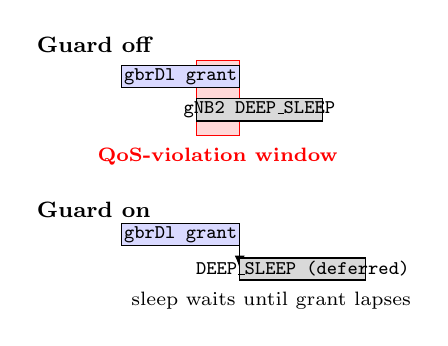
\begin{tikzpicture}[font=\footnotesize]
  \node[font=\footnotesize\bfseries,anchor=west] at (0,1.05) {Guard off};
  \draw[fill=red!30,draw=red,fill opacity=0.5] (2.15,-0.1) rectangle (2.7,0.85);
  \draw[fill=blue!15] (1.2,0.5) rectangle (2.7,0.78);
    \node[font=\scriptsize] at (1.95,0.64) {\ttfamily gbrDl grant};
  \draw[fill=black!15] (2.15,0.08) rectangle (3.75,0.36);
    \node[font=\scriptsize] at (2.95,0.22) {\ttfamily gNB2 DEEP\_SLEEP};
  \node[red,font=\scriptsize\bfseries,anchor=north] at (2.42,-0.14) {QoS-violation window};

  \node[font=\footnotesize\bfseries,anchor=west] at (0,-1.05) {Guard on};
  \draw[fill=blue!15] (1.2,-1.5) rectangle (2.7,-1.22);
    \node[font=\scriptsize] at (1.95,-1.36) {\ttfamily gbrDl grant};
  \draw[-{Latex},thin] (2.7,-1.36) -- (2.7,-1.8);
  \draw[fill=black!15] (2.7,-1.94) rectangle (4.3,-1.66);
    \node[font=\scriptsize] at (3.5,-1.8) {\ttfamily DEEP\_SLEEP (deferred)};
  \node[font=\scriptsize,anchor=west] at (1.2,-2.2) {sleep waits until grant lapses};
\end{tikzpicture}%
}
\caption{SignalViz conflict-timeline view. With the guard off, the
\texttt{gbrDl} grant and \texttt{DEEP\_SLEEP} overlap on gNB2 (QoS-violation
window); with the guard on, the sleep is deferred until the grant lapses. A
live screenshot replaces this schematic in the camera-ready.}
\label{fig:tl}
\end{figure}

\begin{thebibliography}{1}
\bibitem{ts23288} 3GPP, ``Architecture enhancements for 5G System (5GS) to
support Network Data Analytics Services,'' TS~23.288, Rel-18.
\bibitem{ts29574} 3GPP, ``5G System; Data Collection Coordination and Delivery
Services; Stage 3,'' TS~29.574 (Ndccf).
\bibitem{wadud} A.~Wadud, F.~Golpayegani, and N.~Afraz, ``xApp-Level Conflict
Mitigation in O-RAN, a Mobility Driven Energy Saving Case,'' arXiv:2411.03326,
2024.
\bibitem{pacifista} P.~Brach del Prever \emph{et al.}, ``PACIFISTA: Conflict
Evaluation and Management in Open RAN,'' \emph{IEEE Trans. Mobile Computing},
2025.
\bibitem{tr38864} 3GPP, ``Study on network energy savings for NR,'' TR~38.864,
Rel-18.
\bibitem{llmnwdaf} L.~Daniel \emph{et al.}, ``LLM-Enabled NWDAF: A Step Toward
AI-Native 6G Network Intelligence,'' arXiv:2606.11877, 2026.
\end{thebibliography}

\end{document}
